\section{DiscoverySpace: Action Suggestions}
This section describes the Discovery\-Space interface (\autoref{fig:discoveryspace_interface}) and its keyword-based suggestion algorithm.

\begin{figure}[b!]
\centering
  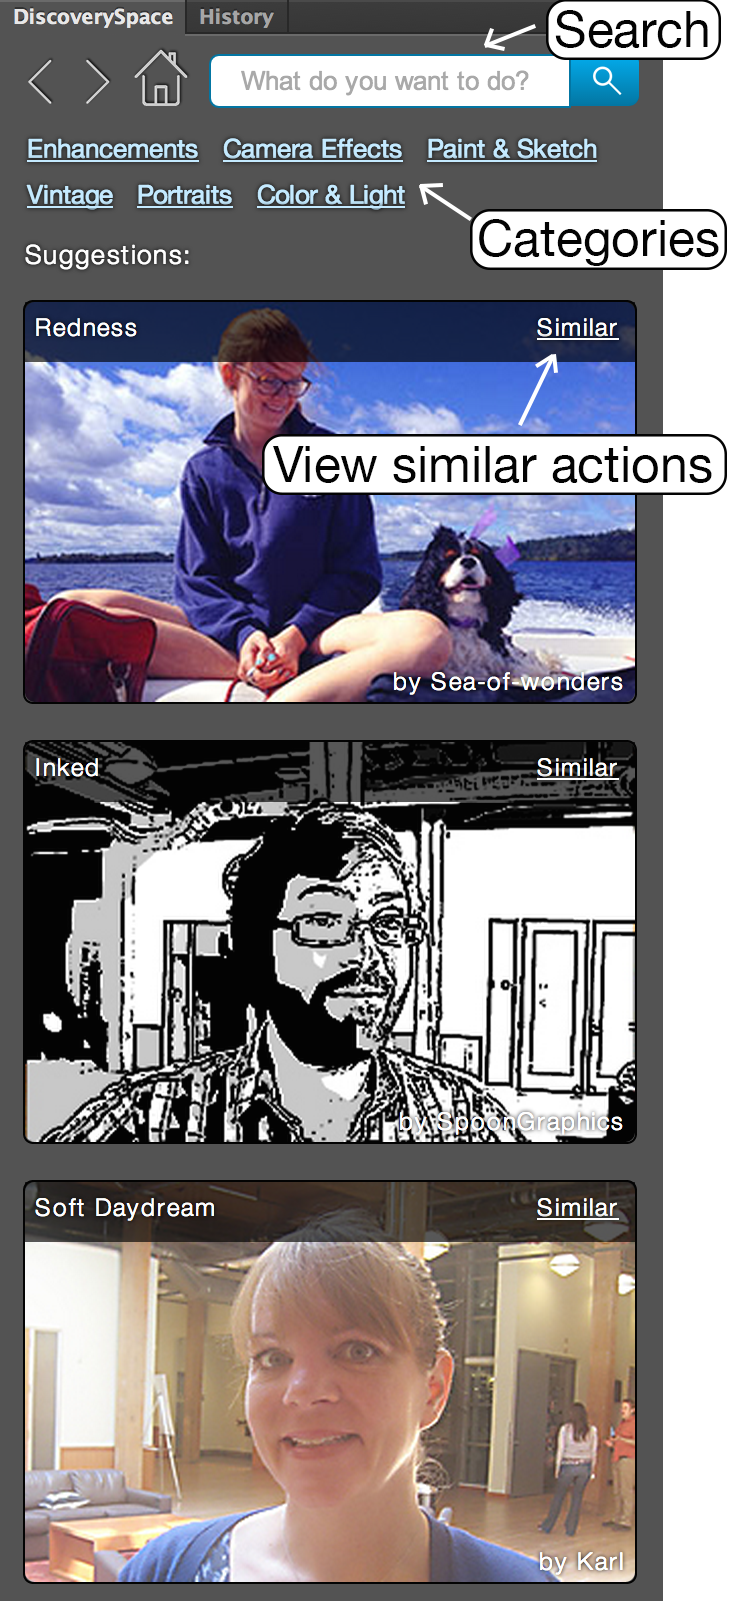
\includegraphics[width=0.35\textwidth]{discoveryspace/figures/discoveryspace_with_labels.png}
  \caption{DiscoverySpace as a panel in Photoshop. Users can apply a suggested action by clicking on its image.}~\label{fig:discoveryspace_interface}
\end{figure}

\subsection{User Experience}
When a user first opens a photo, Discovery\-Space prompts them to enter a goal and select features their image contains from a list (\textit{e.g.} ``contains people'', ``outdoor''). Next, the Discovery\-Space home page appears, containing a search bar, category buttons, and suggested effects (\autoref{fig:discoveryspace_interface}). Each suggestion is displayed by showing the effect applied to an example image with appropriate content. For example, the image for a ``skin smoothing'' effect is of a close-up face. The user can mouse over the image to compare \textit{before} and \textit{after}. Clicking a suggestion applies that action to the photo. As given, the user has no control over the settings for each step of the action; they can see the sequence of steps that was done after applying it by opening the History panel (\autoref{fig:discoveryspace_history}), but cannot step through it or adjust the parameters of individual operations. These actions are therefore intended to allow users to quickly achieve an effect without needing to manually complete all of the intermediate steps. The user can easily undo or redo the effect once it has been applied. If the user scrolls down on the main page, more suggestions appear. To browse suggested effects in a specific category, the user can click a category button. To search the corpus of effects, the user can enter a query in the search bar. The user can also browse effects that are similar to a selected effect by clicking the ``\textit{Similar}'' button on the effect. 

\begin{figure}[b!]
\centering
  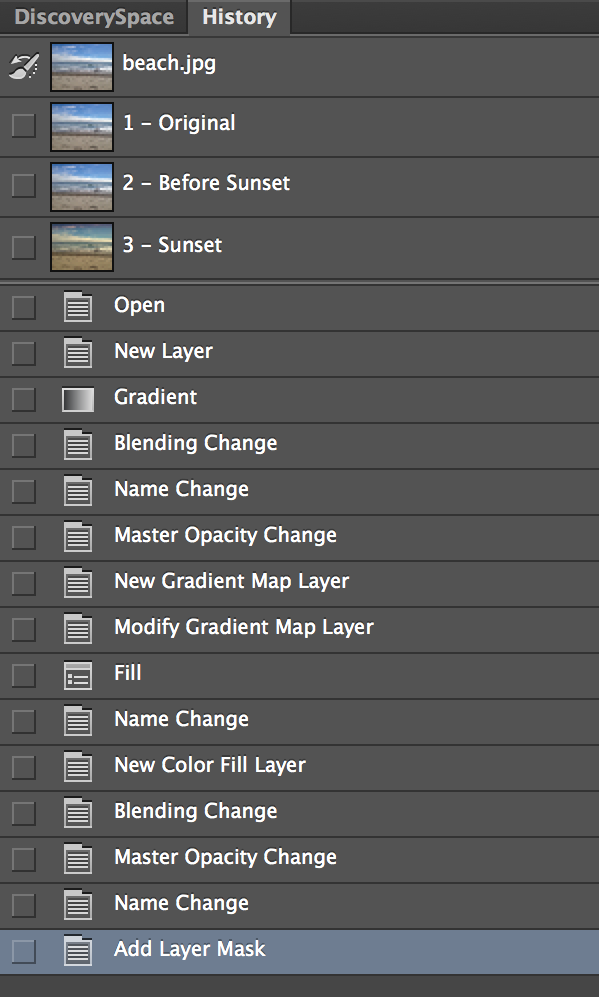
\includegraphics[width=0.35\textwidth]{discoveryspace/figures/history.png}
  \caption{In the History panel, users can review the operations an action has performed.}~\label{fig:discoveryspace_history}
\end{figure}

\subsection{Implementation}
Discovery\-Space is a Photoshop extension panel, written in HTML, Javascript, and Adobe ExtendScript. It retrieves a manually-curated corpus of 115 actions stored on an Amazon S3 server, providing the flexibility to update the actions to reflect popular trends. We manually defined the action categories by reviewing and clustering free actions found online. We created the corpus by downloading 2-3 actions from each subcategory. Paid actions could be added in the future by allowing users the option to pay for effects from within the panel. Discovery\-Space automatically augments search queries with synonyms to maximize the number of relevant results.

\subsection{Keyword-based Recommendations}
Discovery\-Space recommendations take the user's photo as input (\autoref{fig:discoveryspace_rec_alg}). Each action has been assigned a number of descriptive keywords. When opening a new photo, users must select features that describe the image; image analysis could automate this step in the future. We map the selected features to potentially relevant keywords, and assign each action a weight based on the number of matching keywords.

\begin{figure}[b!]
\centering
  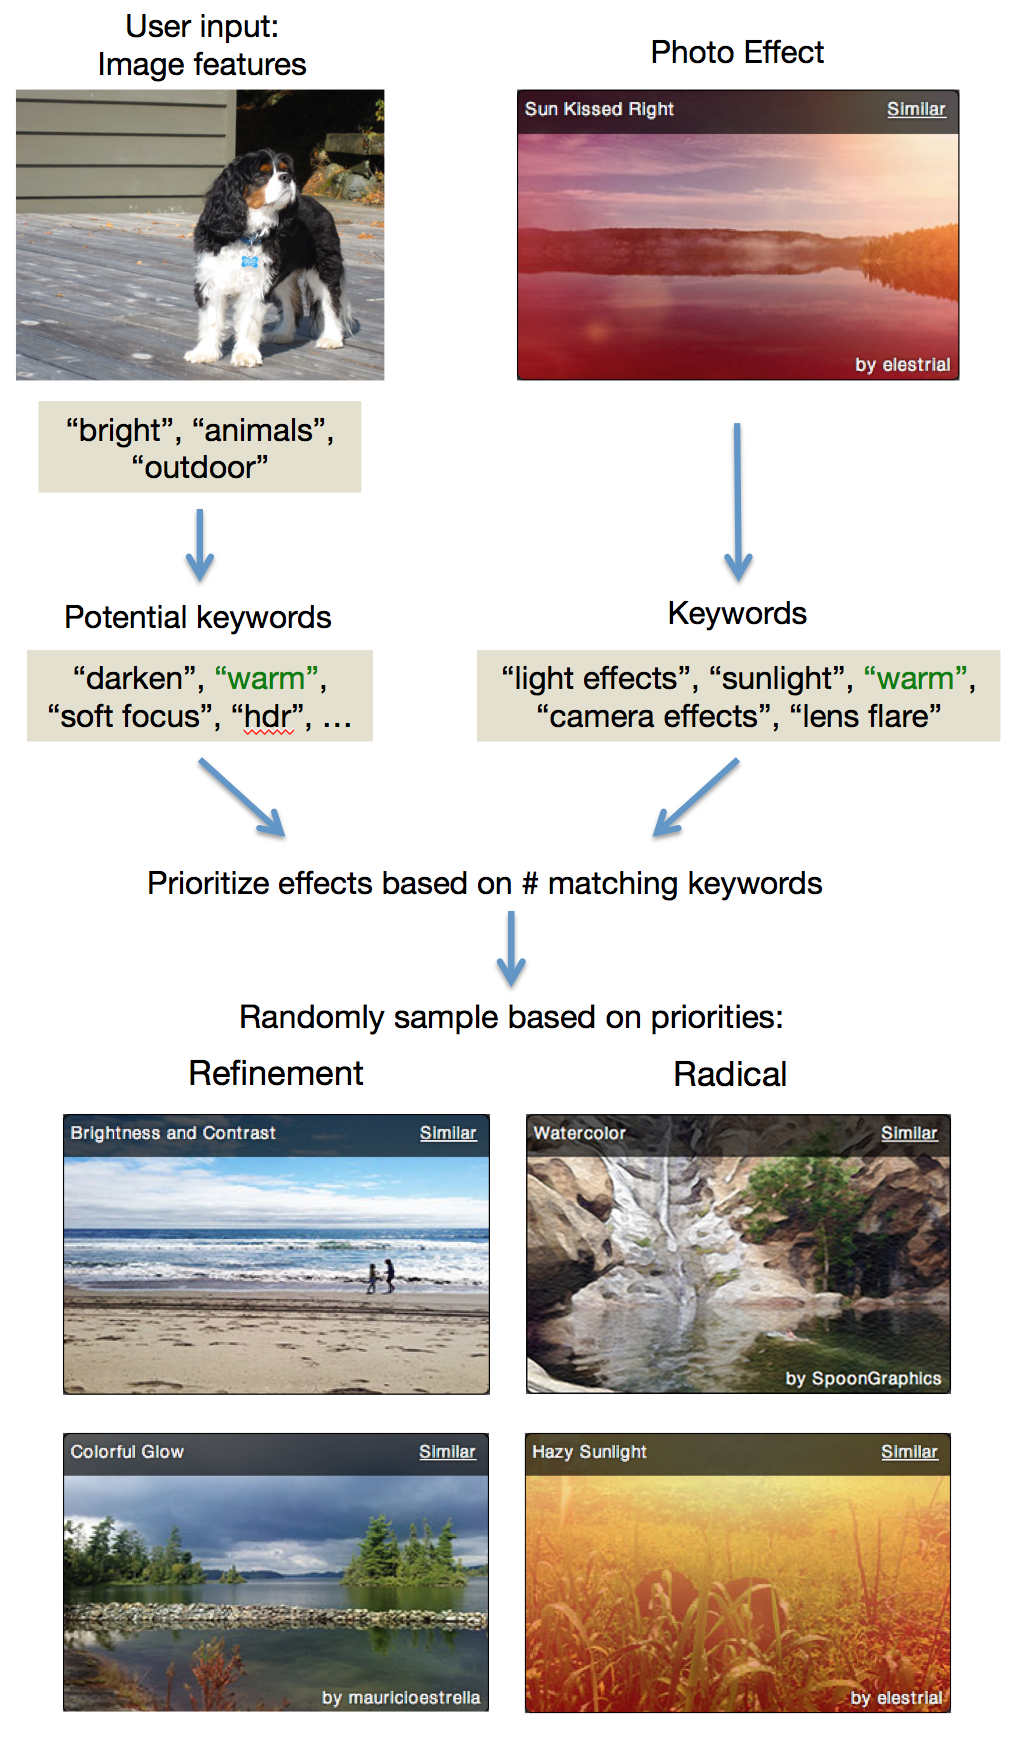
\includegraphics[width=0.6\textwidth]{discoveryspace/figures/rec_alg_new.png}
  \caption{An overview of our keyword-based recommendation algorithm. User-selected image features are mapped to keywords and matched against the keywords for each action in the corpus.}~\label{fig:discoveryspace_rec_alg}
\end{figure}

To select and present suggestions, our algorithm randomly samples from the collection of actions based on these weights: actions with a larger weight have a higher probability of being selected. The randomness encourages discovery by presenting new suggestions when the user refreshes the page. Each action has also been manually classified as either \textit{refinement} or \textit{radical}. An action is deemed \textit{radical} if it produces a drastic effect, does not necessarily maintain realism, and/or takes multiple steps to accomplish. Examples include painting effects, HDR, replicating old cameras, and drastic color effects. An action is deemed a \textit{refinement} if it involves a small adjustment that is meant to improve the photo while maintaining realism, or could be accomplished in one step. Examples include brightening, softening skin, sharpening, and slight color casts. We prefer that both types of effects are suggested, to promote variety in the options. To ensure this, we run the prioritization algorithm separately on the two collections of actions, and then, for every four actions that are suggested, we sample two from the refinement pool and two from the radical pool. This is because on a 27-inch desktop display, Discovery\-Space in its default position shows four suggestions at a time.
